
\documentclass[journal]{IEEEtran}
\usepackage[brazil]{babel}
\usepackage[utf8]{inputenc}
\usepackage[pdftex]{graphicx}

\begin{document}
	
%Titulo do artigo
\title{Controle e supervisão de um sistema de caldeira simulado}

%Nomes dos autores
\author{José Matheus Soares Ferreira 1~Jonatas Mendinça de Vasconcelos Brito 2~Thiago Marques Sousa 3~Daniel Alan Masquita de Vasconcelos4% <-this % stops a space
\thanks{A. 1, Universidade Federal do Ceará, Sobral, Brasil, matrícula:412564}% <-this % stops a space
\thanks{A. 2, Universidade Federal do Ceará, Sobral, Brasil, matrícula:422569}% <-this % stops a space
\thanks{A. 3, Universidade Federal do Ceará, Sobral, Brasil, matrícula:412645}% <-this % stops a space
\thanks{A. 4, Universidade Federal do Ceará, Sobral, Brasil, matrícula:422104}
}

% The paper headers
\markboth{SBL0092 - SOFTWARE EM TEMPO REAL}%
{Shell \MakeLowercase{\textit{et al.}}: Bare Demo of IEEEtran.cls for IEEE Journals}


% make the title area
\maketitle

% As a general rule, do not put math, special symbols or citations
% in the abstract or keywords.
\begin{abstract}
Escreva um breve resumo sobre o trabalho...
\end{abstract}

% Note that keywords are not normally used for peerreview papers.
\begin{IEEEkeywords}
Caldeira, controle de sistema, software em tempo real.
\end{IEEEkeywords}

\IEEEpeerreviewmaketitle

\section{Introdução}


\IEEEPARstart{s}{oftware} em tempo real, pode ser entendido como sistemas computacionais com requisitos de tempo real, sendo uma categoria especial de sistema operacionais. Essa técnica, aplica-se a problemas que exijam requisitos com funcionalidades de natureza temporal não triviais, nesse sentido é essencial a confiabilidade no tempo de execução da tarefa e compatibilidade com prazos e requisitos definidos, ocasionando em resultados corretos logicamente e temporalmente.\cite{IEEEhowto:romulo}

Para os requisitos temporais, é necessário destacar que estão diretamente acoplados ao meio, no sentido de estarem fortemente associados com o mundo físico e que por isso a extração dos requisitos devem ocorrer na perspectiva do sistema responder ao estímulos do ambiente. Destacam-se os seguintes requisitos temporais:  periodicidade, o Deadline, Atualidade ou frescor dos dados e a simultaneidade dos dados.\cite{IEEEhowto:romulo}

Na aplicação de softwares de tempo real, a sincronização e a comunicação entre tarefas pode ocasionar inconsistência de dados e inversões de prioridades entre tarefas caso seja mal implementado. Para os trechos do código onde a tarefa acessa algum recurso compartilhado entre várias tarefas, é necessário definir uma seção crítica. Para evitar a inconsistência dos dados é usado o mecanismos do Mutex, "técnica de sincronização que possibilita assegurar o acesso exclusivo (leitura e escrita) a um recurso compartilhado por duas ou mais entidades"\cite{IEEEhowto:Borges}, evitando que duas tarefas acessem ao mesmo tempo o memória. 

Nesse sentido, para acessar recursos compartilhados por outras tarefas é necessário definir mecanismos de sincronização para controlar o acesso de recursos e garantir que todos as tarefas possam executar suas seções críticas sem interferir com as seções críticas das outras tarefas.

A idéia do monitor é tornar determinados recursos privativo as tarefas \cite{IEEEhowto:romulo}.
\section{Metodologia}

Apresente como o trabalho foi realizado, falando da Parte I e II da descrição. 

Use diagrama de blocos se possível para indicar as etapas realizadas no trabalho.

\section{Resultados e discussões}

Apresente os resultados da parte I e II e discuta os resultados de acordo com o que foi pedido. Veja o exemplo de como colocar imagens no artigo. A Figura \ref{fig1} ...

	\begin{figure}[h]
	\centering
	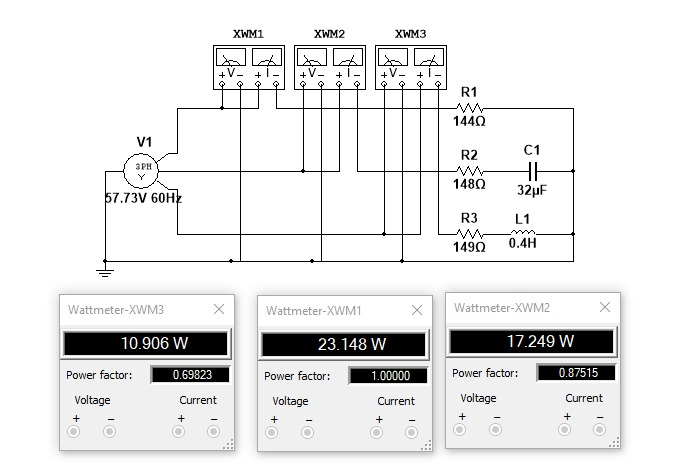
\includegraphics[width=3.5in]{Imagens/medidas.jpg}	
	\caption{Gráfico com as medições realizadas, na ordem dos casos de teste.}
	\label{fig1}
\end{figure}

%%%%%%%%%%%%%%%%%%%%%%%%%%%%%%%%%%%%%%%%%%%%%%%%5
%%%%%%%%%%%%%%%%%%%%%%%%%%%%%%%%%%%%%%%%%%%

\ifCLASSOPTIONcaptionsoff
  \newpage
\fi

\begin{thebibliography}{1}

\bibitem{IEEEhowto:romulo}
Oliveira, R. S. Fundamentos dos Sistemas de Tempo Real. Original registrado na Biblioteca Nacional. Primeira edição, revisão 3, outubro de 2018. ISBN-13: 9781728694047.

\bibitem{IEEEhowto:Borges}
Borges, V. B. Exclusão mútua (mutex). Departamento de Sistemas Eletrônicos Escola Politécnica da USP. 2017.

\end{thebibliography}

%%%%%%%%%%%%%%%%%%%%%%%%%%%%%%%%%%%%%%%%%
%Se tiver foto use essa forma
%%\begin{IEEEbiography}[{\includegraphics[width=1in,height=1.25in,clip,keepaspectratio]{Imagens/autor1.png}}]{Autor 1}
%%Texto da biografia aqui...
%%\end{IEEEbiography}




\end{document}
